
%! FerriganHash.tex
%! Author = Vincent Ferrigan <ferrigan@kth.se>
%! Date = 2022-10-20


% Preamble
\documentclass[a4paper, 11pt]{article}
% Packages
\usepackage[T1]{fontenc}
% \usepackage[utf8]{inputenc} % ska den tas bort iom lua?
% \usepackage[utf8]{luainputenc}
\usepackage[english]{babel}
\usepackage{fontspec}
\usepackage{microtype}
\setmonofont{DejaVu Sans Mono}[Scale=MatchLowercase]
\usepackage{listings}
\usepackage{minted}
\usepackage{latexsym,exscale,stmaryrd,amsmath,amssymb}
\newtheorem{definition}{Definition}
\usepackage{unicode-math}
\usepackage{lmodern}
\usepackage{enumitem}
\usepackage{subcaption}
\usepackage{graphicx}
\usepackage{hyperref}
\usepackage{multirow}
\usepackage{diagbox} % For diagonal lines in tabular
\usepackage{booktabs}
% \usepackage{paralist}

%% Om jag vill referera till ett kod verb av något slag, som void null Int etc
% \usepackage{tcolorbox}
% \newtcbox{\somestuffstyle}{on line,boxrule=0pt,boxsep=0pt,colback=lightgray,top=1pt,bottom=1pt,left=1pt,right=1pt,arc=0pt,fontupper=\ttfamily}

\usepackage[
    backend=biber,
    % hyperref=true,
    maxnames=3, 
    minnames=1, 
    nohashothers=false
    bibencoding=utf8, % eventuellt
    style=apa,
    % citestyle=apa,
    pluralothers=true,
    natbib=true
    % sorting=nyt
    % autocite=inline
    ]{biblatex}
\DefineBibliographyStrings{english}{andothers={et. al}, and={&}}
\DeclareLanguageMapping{english}{english-apa}
\addbibresource{references.bib} % hör till referenser
% \addbibresource{../references.bib} % hör till referenser
% \usepackage[backend=biber,style=apa,natbib=true,sorting=nyt]{biblatex}
% \addbibresource{references.bib}
% \usepackage{natbib}
\usepackage{csquotes}
\usepackage[nottoc]{tocbibind}
\usepackage{xcolor}
\usepackage{siunitx}
\usepackage{tikz}
\usepackage[font=small,labelfont=bf]{caption}
% Addiding JuliaMono
\newfontfamily \JuliaMono {JuliaMono-Regular.ttf}[
    Path      = ./,
    Extension = .ttf
    ]
\newfontface \JuliaMonoMedium{JuliaMono-Regular}
\setmonofont{JuliaMonoMedium}[
    Contextuals=Alternate
]
\usetikzlibrary{matrix, positioning}
\tikzset{
node of list/.style = { 
             draw, 
             fill=gray!20, 
             minimum height=6mm, 
             minimum width=6mm,
             node distance=6mm
   },
link/.style = {
     -stealth,
     shorten >=1pt
     },
array element/.style = {
    draw, fill=white, 
    minimum width = 6mm,
    minimum height = 10mm,
}
}

% \def\LinkedList#1{%
%   \foreach \element in \list {
%      \node[node of list, right = of aux, name=ele] {\element};
%      \draw[link] (aux) -- (ele);
%      \coordinate (aux) at (ele.east);
%   } 
% }
\def\LinkedList#1{%
  \foreach \element in \list {
     \node[node of list, right = of aux, name=ele] {\element};
     \node[node of list, name=aux2, anchor=west] at ([xshift=-.4pt] ele.east) {};
     \draw[link] (aux) -- (ele);
     \coordinate (aux) at (aux2);
   }
   \fill (aux) circle(2pt);
}

\title{Hash tables\\ \small{ID1021 Algorithms and Data structures}} %%TODO VILKEN RUBRICERING
\author{Vincent Ferrigan}

\date{\today}

\begin{document}
    \maketitle
    \section*{Introduction}
    \label{sec:introduction}
    In this study, the performance and mechanism of \emph{Hash Tables}, a 
    data structure supporting \emph{Symbol Tables}, 
    also known as \emph{Dictionaries}, was studied and analyzed.
    Besides comparing the different ways of storing data in Hash Tables,
    the dictionary operations \emph{insertion} and \emph{search} were also compared
    with storing data in the more basic data structure, like \emph{linked lists} and \emph{arrays}, 
    with their equivalent algorithms \emph{Linear Search}, \emph{Binary Search} and 
    \emph{Direct Addressing}. 
    (The latter being more of a ''simple technique'' of storing or
    ''addressing data'' in memory rather than an algorithm.) 
    
    The above-mentioned comparisons were done through different types of benchmarking. 
    The author's intent is to reach certain conclusions regarding 
    the balance between the time and space complexity of hash tables. 

    \section*{Methods}
    \label{sec:methods}
    All the Data Structures and Algorithms were implemented in \emph{Julia}.
    The Code was mostly written in \emph{VSCode} and run on \emph{Julia 1.8.0}.
    Quick-fixes and editing was, however, done in \emph{Vim}. 
    Some scripts were executed from the \emph{REPL terminal},  while others (e.g.
    when using data frames, performing benchmarks and producing plots) 
    were executed from the \emph{Jupyter Notebook}. 
    % Ska jag lägga till länk till min github? To follow the progress.....
    % men då måste notebooken läggas upp.
    
    \subsection*{Tools and packages}
    All tests were performed with the built-in package \emph{Test} and 
    iterative development was made possible through 
    \emph{Revise.jl} -- the latter operates by continuously
    scanning the source code for changes, even changes in functions defined in
    other modules (including modules written in different files). 
    Version control was done through \emph{Git} and \emph{Git-Hub} and the paper
    was written in \emph{\LaTeX} and compiled with \emph{LuaTeX} and \emph{Biber}.
    
    The benchmark data was constructed, manipulated and visualized through
    \emph{DataFrames.jl} and \emph{Plots.jl}, 
    while readable formatting was produced through 
    \emph{Formatting.jl} and \emph{Unitful.jl}. 

    \subsection*{The JIT}
    Julia has a just-in-time (JIT) compilation -- which means that the code is
    dynamically compiled during program run time.     
    It takes time for the JIT compiler to 
    initially load the code and compile it. Therefore, in order not to skew the
    results, \emph{warm-up calls} were performed on certain parts of the code
    before they were benchmarked. This to avoid including 
    compilation time. The warm-up calls were done with the @timed macro prior to
    benchmarking.

    \section*{The Data Structure and their operations} %% TODO CHANGE DEPENDING ON ASSIGNMENT
    This section briefly describes Hash Tables - a data structure that supports
    \emph{Symbol Tables} -- also known as \emph{Dictionaries}. 
    For clarity, the reader will be given an account of the mechanism 
    behind storing data, \emph{values}, in a table 
    that later can be looked up with a \emph{key}. 
    The subsections will go through the key differences between 
    \emph{Direct-}, \emph{Open-} and \emph{Closed Addressing} and their
    \emph{collision resolution} techniques when mapping keys to values; 
    \emph{Chaining} with singly linked lists
    and \emph{Linear Probing}. 
    
    The reader will also be provided with code examples when necessary. 
    A table of Swedish Zip Codes will be used as case study. These
    5-digit postal codes (postnummer) range from $11115$ to $98499$, the lowest
    targets Stockholm, while the highest is located in Pajala. 
    
    \subsection*{1-based indexing and other Conventions}
    \label{subsec:convensions}
    It is important for the reader to note that Julia uses a \emph{one-based-numbering
    convention}, (i.e. array indices start from 1 to N) and that one dimensional
    arrays are called vectors.  
    For consistency, the author has chosen to refer to one dimensional
    arrays as vectors and apply the 1-based convention when numbering
    sequences of elements more broadly. \emph{Modular hashing} 
    will therefore differ -- 
    returning a value in the range $(0,y]$ rather than $[0,y)$. E.g.
    \mintinline{julia}{mod1(11, 11)} returns $11$ and not $0$. This also
    applies when wrapping around vector indices during \emph{linear probing}
    and \emph{hash table resizing}.
        
    Unlike other languages, Julia objects cannot be ''null'' by default. The
    equivalent of \lstinline[language=Python]{None} in Python or
    \lstinline[language=C]{NULL} and \lstinline[language=C]{void} in C is
    \mintinline{julia}{Nothing}. The Julia convention is to return the value
    \mintinline{julia}{nothing}, which is a singleton instance of type
    \mintinline{julia}{Nothing}, when such a side effect is
    desired. 
    
    Function names that end with a bang (!) mutates the arguments it receives. 
    This name suffix is by convention in Julia. 
    \subsection*{Hashing Tables}
    In a \emph{Direct-address Table}, the indices of a vector directly correspond to the keys that
    data (values) are mapped to. 
    The data object at index $11515$ of the vector would store the information 
    related to zip-code ''115 15'', requiring the program to at minimum allocate 
    memory for a vector of size $98499$. The set of keys that are actually stored 
    is quite small relative to the vector size. 
    Hash tables require a lot less storage. Instead of directly using the key as index,
    the index is computed from the key. A procedure called \emph{hashing}, which maps a key 
    (and its associated value) into a hash table by using a hash function. Simply put, it 
    converts keys into vector indices \parencite{Segeqick2011Alg4th}. 
    
    Several methods can be used for creating hash functions that map keys into slots. 
    The one used in this study is called \emph{The Division Method}, 
    a static approach to hashing that maps key $k$ into one of $m$ slots by taking the remainder of 
    $k$ divided by $m$. In mathematical terms, the  hash function is (\(h(k) = k\mod m\)).
    The result $h(k)$ is called the \emph{hash value} of key $k$ \parencite{CormenThomasH2022ItA}.
    
    \begin{minted}[
        % label=codeexample, 
        % linenos, 
        % breaklines, 
        % frame = single, 
        fontsize=\footnotesize]{julia}
hashing = (key, m) -> hashingByDivision(key, m)
hashingByDivision = (k::Integer, m) -> mod1(k,m)
    \end{minted}
    
    As mentioned earlier, vectors in this study are 1-based, 
    and the returning hash value will therefore be in range $(0,m]$.
    If key $k$ equals $m$, the function \mintinline{julia}{mod1(k,m)}
    returns $m$ and not $0$. The situations where more than one key 
    hash to the same slot, is called a \emph{collision}. This paper 
    studies two types of collision resolution techniques; 
    \emph{chaining}, which is used by \emph{closed address tables}
    and \emph{Linear probing} which is used by \emph{open address tables}.

    \subsection*{Chaining}
    In a \emph{closed address table}, every slot of the hash table is the head
    of a singly linked list. If two keys hash to the same slot, they 
    get ''chained'' together, as illustrated in \autoref{fig:chaining}. 

    \begin{figure}[h]
    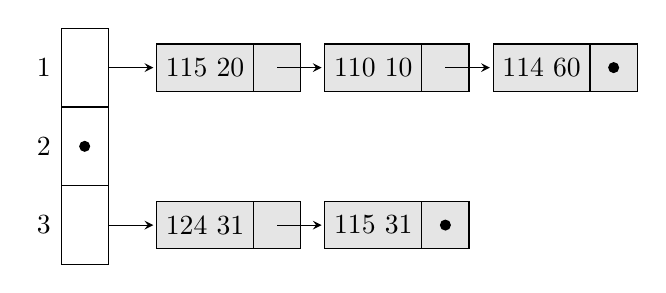
\begin{tikzpicture}
\foreach \index/\list in {1/{115 20, 110 10, 114 60}, 2/{}, 3/{124 31, 115 31}}  
{

   \node[array element] (aux) at (0,-\index) [label=left:\index]{};
   \LinkedList{\list}
}
\end{tikzpicture}
    \caption{Closed Addressing.
Collision resolution by chaining. Each slot of the vector contains a reference
to a singly-linked list containing
key-value pairs with the same hash value.}
    \label{fig:chaining}
    \end{figure}

    In the algorithm that was written for this study,
    the insert method calls a push function to prepend 
    a key to the list that shares the same hash-value (see \autoref{code:closedaddress}).
    The hash value corresponding to the slot, i.e. index of the vector. 

    \begin{figure}[h]
        \centering
    \begin{minted}[
        label= Data Types (Closed Address Hash Table),
        linenos, 
        % breaklines, 
        frame = single, 
        fontsize=\footnotesize]{julia}
mutable struct ClosedAddressHT{K,T} <: HashTable{K,T}
    data::Vector{Union{Nothing, Node{K,T}}}
    m # slot-size
    n # amt of entries
end

mutable struct Node{K,T}
    key::K
    entry::T
    next::Union{Node{K,T}, Nothing}
    size # length of list from current node
end
    \end{minted}
    \begin{minted}[
        label= Insertion by chaining,
        linenos, 
        % breaklines, 
        frame = single, 
        fontsize=\footnotesize]{julia}
function insert!(
    h_table::ClosedAddressHT{K,T},
    key::K,
    entry::T
    ) where {K,T}

    h_value = hashing(key, m(h_table))
    (h_table.data[h_value] 
    = pushfirst!(h_table.data[h_value], key, entry))
    h_table.n += 1
end

function pushfirst!(
    node::Union{Nothing, Node{K,T}}, 
    key::K, 
    entry::T) where {K,T}

    return Node(key, entry, node, (size(node) + 1))
end
    \end{minted}
    \caption{Julia Code example of collision resolution by chaining.} %% TODO ADD CAPTION
    \label{code:closedaddress} %% TODO ADD LABEL
    \end{figure}

    \subsection*{Linear probing}
    In an \emph{open address table}, every key-value pair gets stored inside the hash table. 
    No lists of references are stored
    outside the table. Every slot contains either a key-value pair or \mintinline{julia}{nothing}.
    Collisions are resolved by probing the table for empty slots.
    Probing can be in several ways. This study has been assigned to implement 
    \emph{linear probing} -- which according to \textcite{Segeqick2011Alg4th} is The
    simplest open-addressing hashing method. 
    Simply put, if the slot is occupied, 
    the algorithm linearly probes the next until it locates an empty slot for insertion 
    (see while-loop in \autoref{code:openaddress}).

    \begin{figure}[h]
        \centering
    \begin{minted}[
        label= Data Types (Open Address Hash Table),
        linenos, 
        % breaklines, 
        frame = single, 
        fontsize=\footnotesize]{julia}
mutable struct StaticOpenAddressHT{K,T} <: OpenAddressHT{K,T}
    data::Vector{Union{Nothing, Datum{K,T}}}
    m # slot-size
    n # amt of entries
end

struct Datum{K,T}
    key::K
    entry::T
end
    \end{minted}
    \begin{minted}[
        label= Insertion by linear probing,
        linenos, 
        % breaklines, 
        frame = single, 
        fontsize=\footnotesize]{julia}
function insert!(
    h_table::StaticOpenAddressHT{K,T}, 
    key::K,
    entry::T
    ) where {K,T}

    # load factor α < 1 
    (h_table.m < h_table.n && throw(ArgumentError(
     "Only one slot left in static hash table")))

    pos = hashing(key, h_table.m)
    while !isa(h_table.data[pos], Nothing)
        if isequal(h_table.data[pos], key)
            h_table.data[pos].entry = entry
        end
        pos = mod1((pos + 1), h_table.m)
    end
    h_table.data[pos] = Datum(key, entry)
    h_table.n += 1
end
    \end{minted}
    \caption{Julia Code example of collision resolution by linear probing. 
    The insert method also check for search hits and can therefore be used for
    handling updates} %% TODO ADD CAPTION
    \label{code:openaddress} %% TODO ADD LABEL
    \end{figure}

    Unlike closed address tables, the 
    amount of key-value pairs must never exceed the number of slots. The
    while-loop in the \mintinline{julia}{insert!()} method would be 
    infinite if the hash table would be full. 
    A way to solve this issue is through 
    resizing (and rehashing) the table. Rewriting row 7-9 in the insert method
    to:
    \begin{minted}[
        % label= Insertion by linear probing,
        % linenos, 
        % breaklines, 
        % frame = single, 
        fontsize=\footnotesize]{julia}
if h_table.n > ÷(h_table.m, 2) # load factor α > 1//2
    resize!(h_table, *(h_table.m, 2), typeof(key), typeof(entry))
end
    \end{minted}
    and adding the following function:
    \begin{minted}[
        % label= Insertion by linear probing,
        % linenos, 
        % breaklines, 
        % frame = single, 
        fontsize=\footnotesize]{julia}
function resize!(
    h_table::DynamicOpenAddressHT{K,T}, 
    capacity,
    k_type::DataType, 
    t_type::DataType
    ) where {K,T}
    temp_ht = DynamicOpenAddressHT{k_type,t_type}(capacity)
    for datum ∈ h_table.data
        !isa(datum, Nothing) && insert!(temp_ht, datum.key, datum.entry)
    end
    h_table.data, h_table.m = temp_ht.data, temp_ht.m
end
    \end{minted}

    This resizing and rehashing procedure (together with recommendation on when to use it) 
    will be further elaborated in the discussion \autoref{sec:discussion} below.

    % XXXXXxxxx lägg till searching XXXXXXX

    \clearpage
    \section*{Results}
    \label{sec:results}
    In total, three benchmarks were performed. One small benchmark 
    comparing the running time for two search operations on a direct address table with both 
    linear search and binary search (see \autoref{tab:lookup}). The second 
    measuring collision resolution by chaining (see \autoref{tab:collision}) and
    the third (demonstrated in \autoref{tab:attempts})
    comparing linear probing on tables with different load factors. The latter also comparing open to 
    closed address tables. 
    
    \subsection*{Lookup Benchmark}
    % xxxxxx describe benchmark, ref to \autoref{tab:lookup}


    \begin{table}[h]
        \centering
        \small
\begin{tabular}{lrrrr} % TODO: correct columns
    \toprule
    & \multicolumn{4}{c}{\textbf{Key}} \\\cmidrule(lr){2-5}
    \textbf{Algorithm} & \multicolumn{1}{c}{"115 15"} &\multicolumn{1}{c}{"994 99"}& \multicolumn{1}{c}{\num{11515}}&\multicolumn{1}{c}{\num{99499}}\\
    \cmidrule(lr){1-1}
    \cmidrule(lr){2-5}
    Linear Search      &\SI{14}{\nano\second}   &\SI{32871}{\nano\second}   &\SI{17}{\nano\second}  &\SI{7432}{\nano\second}\\
    Binary Search      &\SI{107}{\nano\second}  &\SI{132}{\nano\second}     &\SI{119}{\nano\second} &\SI{134}{\nano\second} \\
    Direct Addressing  & \multicolumn{2}{c}{n/a}                       &\SI{15}{\nano\second}  &\SI{15}{\nano\second}  \\
    \bottomrule
\end{tabular}
    \caption{A lookup benchmark comparing linear and binary search to a direct address table.
    } % TODO: add caption
    \label{tab:lookup} % TODO: add correct label
    \end{table}

    % \begin{figure}[h] % You can have subfigures !! If necessary 
    %     \centering
    %     \includegraphics[width=0.8\textwidth]{./input/xxxxx.pdf} %% TODO: add pdf
    %     \caption{xxxx}%% TODO: add caption
    %     \label{fig:fig1} %% TODO: add correct fignbr /label
    % \end{figure}
    \subsection*{Collisions}
    % xxxxxx describe benchmark, ref to \autoref{tab:collision}

    \begin{table}[h]
        \centering
        \small
\begin{tabular}{lrrrrrrrr}
\toprule
& \multicolumn{8}{c}{Keys (Slots)}\\
\cmidrule(lr){2-9}
& \multicolumn{4}{c}{Compound} &\multicolumn{4}{c}{Prime}\\
\cmidrule(lr){2-5}
\cmidrule(lr){6-9}
Collisions       & \multicolumn{2}{c}{\num{10000} slots} & \multicolumn{2}{c}{\num{20000} slots} & \multicolumn{2}{c}{\num{9973} slots} & \multicolumn{2}{c}{\num{19997} slots} \\
    \cmidrule(lr){1-1}
    \cmidrule(lr){2-3}
    \cmidrule(lr){4-5}
    \cmidrule(lr){6-7}
    \cmidrule(lr){8-9}

None  & \num{2050} & (\num{2050}) & \num{4180} & (\num{4180}) & \num{3667} & (\num{3667})& \num{5069}& (\num{5069})   \\
One  & \num{2260} & (\num{1130}) & \num{2942} & (\num{1471}) & \num{3764} & (\num{1882})& \num{3132}& (\num{1566})   \\
Two  & \num{1635} & (\num{545})  & \num{1527} & (\num{509})  & \num{1695} & (\num{565}) & \num{1194}& (\num{398})   \\
Three& \num{1336} & (\num{334})  & \num{776}  & (\num{194})  & \num{484}  & (\num{121}) & \num{240} & (\num{60})   \\
Four & \num{1015} & (\num{203})  & \num{250}  & (\num{50})   & \num{65}   & (\num{13})  & \num{40}  & (\num{8})   \\
Five & \num{594}  & (\num{99})   & \num{0}    & (\num{0})    & \num{0}    & (\num{0})   & \num{0}   & (\num{0})   \\
Six  & \num{392}  & (\num{56})   & \num{0}    & (\num{0})    & \num{0}    & (\num{0})   & \num{0}   & (\num{0})   \\
Seven& \num{312}  & (\num{39})   & \num{0}    & (\num{0})    & \num{0}    & (\num{0})   & \num{0}   & (\num{0})   \\
Eight& \num{81}   & (\num{9})    & \num{0}    & (\num{0})    & \num{0}    &(\num{0})    & \num{0}   & (\num{0})   \\
\hline
Empty slots& \num{0}& (\num{5535}) & \num{0}    &(\num{13596}) & \num{0}    &(\num{3725}) & \num{0}   & (\num{12896})\\
\hline
Sum              & \num{9675} & (\num{10000}) & \num{9675} & (\num{20000}) & \num{9675} & (\num{9973})&\num{9675} & (\num{19997})\\
\bottomrule
\end{tabular}
    \caption{Collision data by chaining. Two collisions imply that tree keys share the same
    hash value and are therefore stored in the same slot (also known as bucket).
    In other words, three data objects are chained together as a Singly Linked
    List. 
    For a hash-table that contains \num{10,000} slots, 
    $545$ of them contain 3 keys each. 
    In total $1635$ keys share the same hash value with two other keys.} %
    \label{tab:collision} % TODO: add correct label
    \end{table}

    \subsection*{Attempts}
    % xxxxxx describe benchmark, ref to \autoref{tab:attempts}
    \begin{table}[h]
        \centering
        \small
\begin{tabular}{lrrrrrr}
\toprule
& \multicolumn{6}{c}{Hash Tables}\\
\cmidrule(lr){2-7}
& \multicolumn{3}{c}{Chaining} &\multicolumn{3}{c}{Linear Probing}\\
\cmidrule(lr){2-4}
\cmidrule(lr){5-7}
Attempt & \num{10000} m & \num{9973} m & \num{20333} m & \num{10000} m & \num{9973} m & \num{20333} m \\
\cmidrule(lr){1-1}
\cmidrule(lr){2-7}
First & $4465$ & $6248$ & $7964$ & $2983$ & $4028$ & $7035$\\
Second & $2415$ & $2581$ & $1572$ & $91$ & $140$ & $281$\\
Third & $1285$ & $699$ & $134$ & $119$ & $139$ & $196$\\
4th & $740$ & $134$ & $5$ & $117$ & $97$ & $185$\\
5th & $406$ & $13$ & $0$ & $91$ & $152$ & $92$\\
6th & $203$ & $0$ & $0$ & $70$ & $89$ & $147$\\
7th & $104$ & $0$ & $0$ & $83$ & $84$ & $93$\\
8th & $48$ & $0$ & $0$ & $103$ & $86$ & $92$\\
9th & $9$ & $0$ & $0$ & $85$ & $95$ & $81$\\
10th & $0$ & $0$ & $0$ & $79$ & $52$ & $109$\\
\multicolumn{7}{l}{.}\\
\multicolumn{7}{l}{.}\\
20th & $0$ & $0$ & $0$ & $50$ & $45$ & $49$\\
30th & $0$ & $0$ & $0$ & $27$ & $4$ & $14$\\
100th & $0$ & $0$ & $0$ & $3$ & $1$ & $2$\\
300th & $0$ & $0$ & $0$ & $4$ & $0$ & $0$\\

\bottomrule
\end{tabular}
    \caption{Number of keys per attempt. \num{10000} is a compound number while both \num{9973} and \num{20333} 
    are prime. The first prime gives a load factor close to $1 \alpha$
    while the second generates a load factor that is less than $\frac{\alpha}{2}$.
    } %
    \label{tab:attempts} % TODO: add correct label
    \end{table}

    \clearpage
    \section*{Discussion}
    \label{sec:discussion}
    As confirmed by \autoref{tab:lookup}, binary search has a time complexity of $O(\log n)$,
    while the running time for linear search is linear. However, unlike for binary search, 
    linear search doesn't require data to be ordered. 
    Adding data to an unsorted vector is performed in constant time, but if obtaining 
    an order is required, as is the case for binary search,  
    the time complexity becomes linear. Apart from that, the data has to be sorted
    to begin with. Which at best can be performed by another algorithm with a 
    time complexity of $O(\log n)$. Using a table, however, is linear. 
    With a direct addressed table, both search and insert operations only 
    require constant time. For large data the space complexity 
    would be far to great to make direct addressing a feasible solution.  
    A hash table, on the other hand, requires much less storage and can, in theory, still 
    run search and insert operations at constant (amortized) time \parencite{Segeqick2011Alg4th}.
    The challenge is to try to find the right balance between time and space.
    There are several factors that play a role. 
    For example, the worst case for open hashing (i.e. by chaining) could lead to a 
    search time complexity of $0(n)$. The wrong hash function could 
    hash all keys to the same bucket. Basically resulting in a structure that is no better 
    than a linked list. So, what makes a good hash function? Apart from being fast to compute 
    and consistent, a hash function should distribute the keys as uniformly as possible.  
    For the hashing method that was used in this study, 
    the recommendation from both 
    by \textcite{Segeqick2011Alg4th} and \textcite{CormenThomasH2022ItA}
    is to take $m$ to be a prime not too close to a power of $2$. Which in fact 
    was validated by the last two benchmarks in \autoref{tab:collision} and
    \autoref{tab:attempts}. 
    Compare the closed address table of size \num{9973} with \num{10000}.  
    38 percent of all keys in the closed address table 
    had no collisions when the size of the table was prime, while adding seven more slots would
    decrease the number to 21 percent. Roughly 57 percent of all slots are empty compared 
    to $38$ percent if the size is prime. No keys have more than four other keys chained to it 
    in a table of $9973$ slots while $1379$ do in a table of \num{10} thousand buckets. 
    As the data in \autoref{tab:collision} also implies, constraining the size of the hash table 
    to a prime has a greater impact than increasing it size.
    However, data in linked lists are not linearly placed in memory, which
    results in cache-misses and therefore performance degradation. 
    Open addressing could increase the number of cache hits, where linear probing 
    is considered being the simplest approach \parencite{CormenThomasH2022ItA}. 
       
    Nevertheless, spreading the data too greatly negatively
    impacts their degree of spatial locality in memory. Which decreases the 
    likelihood of cache hits during a long linear probe sequence. For linear probing, 
    the ratio $\alpha = \frac{n}{m}$ has a great impact. 
    A ratio known as a hash tables \emph{load factor}. 
    Where $n$ is the number of elements stored in the table and $m$ is the number of slots. 
    Since each slot can only hold one key, the load factor can never be greater than one. 
    A hash table must also never be full, since it would result in an infinite loop during probing. 
    For good performance, it is recommended to stay between one-eighth and one-half. According 
    to \textcite{Segeqick2011Alg4th}, when the load factor is about one half, 
    the average number of probes for a search hit is about $1.5$ and $2.5$ for search miss. As 
    the data in \autoref{tab:attempts} shows, 
    the majority of keys in a table with a load factor close to 1 require more than 10 attempts (or steps)
    to be located, while only one quarter do for a table with a load factor of one half. There are 
    several other techniques to improve this figure, one requiring better hashing functions. 
    Deleting an item is also an issue. Replacing the deleted key with ''nothing'' might result in 
    a prematurely terminated search. One way of solving this in Julia, might be  
    replacing the newly freed slot with the singleton \mintinline{julia}{missing}, or,
    with a trickier process suggested by \textcite{Segeqick2011Alg4th}, reinserting into 
    the table all the keys in the cluster that are below the deleted key. Which might
    increase future cache hits.
  

\printbibliography
\end{document}